\documentclass[10pt,twocolumn]{article}

% use the oxycomps style file
\usepackage{oxycomps}
\usepackage{graphicx}

% usage: \fixme[comments describing issue]{text to be fixed}
% define \fixme as not doing anything special
\newcommand{\fixme}[2][]{#2}
% overwrite it so it shows up as red
\renewcommand{\fixme}[2][]{\textcolor{red}{#2}}
% overwrite it again so related text shows as footnotes
%\renewcommand{\fixme}[2][]{\textcolor{red}{#2\footnote{#1}}}

% read references.bib for the bibtex data
\bibliography{references}

% include metadata in the generated pdf file
\pdfinfo{
    /Title (Comps Final)
    /Author (Connor Wierman)
}

% set the title and author information
\title{Comps Final - Uni-Housing}
\author{Connor Wierman}
\affiliation{Occidental College}
\email{https://www.overleaf.com/4479452845bmywvrtxqnkj}

\begin{document}

\maketitle

\section{Introduction and Problem Context}
\subsection{Societal Context}
College students face some of the most challenging living situations in the country. With their unique moving patterns, typically moving in during August or September and moving out in May or June, finding desirable or even acceptable housing can be difficult. There are currently 12 million full-time college students, and it is estimated that about 75 percent of them live away from home. Among these 9 million students, 20 percent struggle to find stable housing during the school year, when university housing options are more readily available \cite{CNBC}. The situation can also apply to summer months if students are unable to return home and must find short-term accommodations for jobs or internships.

The most desirable solution to this problem would be to just fix the housing crisis. I would love the opportunity to use public policy to rewrite zoning laws, increase housing supply and build more university housing. Unfortunately I am not in the position to fix those issues, and for the most part those problems do not appear to be going away anytime soon. However, an issue I do believe I can fix using this application is the high vacancy rate we see in housing across the country today. 11.6 percent of all housing is vacant, but more importantly a staggering 5.8 percent of rental units remain without a tenant. \cite{AnytimeEstimate} These are investment units that no one wants to have empty yet remain unoccupied. 

These challenges are also personal to me. As a student at Oxy, I was reluctant to live in a dorm for my third consecutive year but found my options for off-campus housing limited due to negative biases against college students or a lack of marketing to connect students with interested landlords. This issue even led to a friend of mine spending the first week of the school year in a hotel due to the difficulty of finding housing as a college student in the Eagle Rock area. In addition, growing up in a small town just north of Tucson, AZ, I found myself seeking internship opportunities in nearby cities that offered more opportunity to pursue my chosen career path such as Phoenix, where a daily commute was not feasible. Even though my internship was across the street from Arizona State University, I still had difficulty finding temporary housing. My personal experience along with the testimony of millions of college students shows that finding housing as a college student can prove to be a burdensome and frustrating experience.

On the other hand, homeowners who rent to college students can benefit from this market as well, and are currently doing a very poor job connecting with this large group of possible clientele. Despite perceived risks, renting to college students can result in higher rental yields, increased profits through room-by-room rentals, and high demand, as most universities cannot house all their students \cite{FortuneBuilder}. Furthermore, college rentals make excellent investment properties due to students' generally low expectations, which can result in lower maintenance and overall costs. \cite{zaransky2006profit} In summary this is a problem that needs to be addressed, not only could it contribute to bringing down housing insecurity, an application that improves the college housing search process would at a minimum have the opportunity to make one of the most stressful parts of every year for a college student a bit easier. 

\subsection{Technical Context}
While my main motivation for the creation of this app is attempting to contribute to a problem I have personally dealt with, from a the perspective of a Computer Science Undergraduate it is an interesting project given the variety of fields it covers. This project allowed me to combine various technical aspects, such as front-end development and API integration, to create a practical prototype for a real-world problem. Addressing the unique housing needs of college students presents a challenge that requires a thorough understanding of existing technologies, as well as the ability to innovate and customize a platform tailored to a specific audience. As a senior computer science student, this project offers me an opportunity to apply my knowledge and skills in a meaningful way, while also pushing me to learn and explore new tools and technologies. 

\section{Technical Background}
In this section I aim to provide an overview of the technical knowledge necessary to understand my Uni-Housing web application project. By assuming the reader is a CS undergraduate, I will introduce essential terminology and concepts related to web development and the project as a whole. Many of these I had to investigate myself as they were not terms I was familiar with before beginning my research.

\noindent Web Development: Web development involves creating websites or web applications that can be accessed through a web browser. It is typically divided into two categories: front end and back end. The front end is the visual part of the website, which includes user interface design, and the back end is responsible for server-side processing and data management. This project focuses almost entirely on the front end given my time and technical limitations. 

\noindent React: React is a popular JavaScript library used for building user interfaces, particularly for single-page applications. It utilizes a component-based architecture, which enables better organization of the code, easier debugging, and efficient rendering. \cite{ReactJS}

\noindent CSS: CSS is a technology used in the creation of websites, used for describing their presentation, including colors, layout, and fonts, separating content from design and improving content accessibility. CSS enables developers to apply style rules to HTML elements or groups of elements efficiently. Modern CSS has evolved to include capabilities such as responsive design, animations, and grid layouts, making it an indispensable tool in creating visually engaging and user-friendly websites. Its widespread adoption and continuous development reflect its vital role in shaping the aesthetic and functional aspects of web applications.

\noindent JavaScript: JavaScript is a widely-used programming language, primarily known for its role in web development. It enables developers to build dynamic and responsive user interfaces, allowing for real-time updates without the need to reload the page. It operates on both in the browser and on the server side, making it a key player in site development. 

\noindent Node.js: Node.js is a tool that lets you run JavaScript in other places besides web browsers. With Node.js, you can write code that works on servers, it can be used for creating websites and online tools that need to manage lots of data. It also comes with npm, or Node Package Manager, which is like a big library of ready-to-use code pieces that make a developer's job easier. Because of all these4 features, Node.js is very popular for building all sorts of things on the internet, from simple websites to complex online services.

\noindent React Router Dom: This library is crucial for managing navigation within the single-page application. It enables seamless transitions between different components without reloading the entire page. This contributes significantly to a smooth and user-friendly experience within the web application.

\noindent Axios: Axios is a promise-based HTTP client used for making API requests. In the application, it plays a vital role in fetching data, it interacts with external services such as the Google Maps Distance Matrix API to calculate distances between properties and user locations.

\noindent API: An API, or Application Programming Interface, is a set of rules and protocols for building and interacting with software applications. APIs enable software systems to communicate with each other, allowing them function with one another easily and securely. They act as intermediaries, allowing one application to access the services or data of another, often over a network. APIs can be used for various purposes, for example in web-based services and cloud applications. They provide a standardized way for applications to request and deliver information, ensuring compatibility and simplifying the process of integrating different software components. By abstracting the underlying implementation details, APIs allow developers to use complex functionalities without needing to understand the inner workings of the systems they are interacting with, facilitating a more efficient and streamlined development process. In this application we will use the Distance Matrix API, a service provided by Google Maps that calculates distances and travel times between origins and destinations. It is particularly useful for applications where such calculations are needed for a number of locations simultaneously.

\noindent User User-Centered Design (UCD): UCD is a design process framework that focuses on the end-users and their needs throughout the build process. This approach involves understanding the who, what, and why of usage by centering the entire development process around the potential users of a product or service. UCD seeks to create solutions that are tailored to the user's goals, requirements, and feedback, rather than forcing adaptation on the part of the user. 

By understanding these key concepts and terminology, you should have the foundational knowledge required to Understand my application uni-housing and the rationale behind the chosen technologies and components.

\section{Prior Work}

The current issues plaguing the college housing market other than a lack of affordable housing, are the lack of sites designed for the housing search needs of college students. College students often find themselves caught between long-term leases that can outlast their desired stay and expensive nightly rentals, like those offered by Airbnb or Vrbo. These options can be overpriced and sometimes lead to unpleasant interactions between renters and owners once the renter's status as a college student is revealed. Discrimination based upon in individual being a student is perfectly legal by the way. \cite{Boston.com} This summer for example I had multiple Air Bnb hosts reject my stay when they discovered my age. 

Existing platforms like Cribwiz attempt to "match" students with suitable housing options using algorithms, but they often fall short in delivering a seamless experience. \cite{cribwiz} For instance, I tried using the service myself and found it to be lacking in effectiveness. I used six of my ten available matches and received only one call about a property after a month of using the service. Furthermore, platforms that explicitly target college students, such as campusrent.com, fail to provide the promised variety of summer subleases and instead showcase generic apartment advertisements.\cite{campusrent}

I believe I can address these issues by developing an app that focuses on students ability to filter to their unique housing preferences and connects them with landlords who have listed housing options that align with prospective tenants desires. The app will be explicitly designed for college rentals and display information most useful to those in the student demographic, most importantly the apps concept as being marketed \textbf{\textit{for students}} will ensure everyone understands the individuals in the transaction from the outset. This approach aims to eliminate misunderstandings and bring in property owners without bias against college students which should provide a more transparent rental process for both students and landlords. Additionally, the current applications monopolize the communication process between renters and landlords. Sites like Zillow, and Amber Student all require inquiry or communication on the site before the transaction members are able to speak directly. \cite{zillow2023} \cite{AmberStudent} Given that these are relatively long term leases and these sites are not offering rental agreements, this adds an additional burden to the transaction for homeowners often pushing them to list their properties in more informal ways such as on Craigslist or Facebook. The negatives with that are that those sites aren't designed to handle fraudulent listings, and they can be dangerous options for students as they are known to be filled with rental scams. \cite{PlaceMeLiving2021} Fixing this issue by providing immediate access to contact information can remove a burden that is preventing listings from being seen by a wider array of possible clientele. 

By focusing on the specific needs and challenges faced by university students in the housing market where previous work fails, my application design has the potential to make an impact on the rental process for this demographic. Ultimately, I hope to improve upon these existing platforms by creating one tailored to college students, and landlords who are interested in tapping into the profitable college rental market by providing them with a reliable, targeted pool of potential tenants.

\section{Methods}
In this section, we will discuss the various procedures I took to understand user needs, before transitioning to the methods and technologies chosen to build my web app. To be clear this is an application with the goal of making the yearly housing search easier for college students. The following paragraphs will delve into the processes of user testing and technical component that shaped the application and how they contribute to the app's overall functionality and user experience.

\subsection{Project Beginnings}
I do think it is important to acknowledge that in the early stages of my project, my primary goal was to develop some level of familiarity with React to ensure I could build the application I was envisioning because I had no prior experience. I also bring this up because this portion of my skill development was in tandem with my first few rounds of user interviews and testing. A significant portion of my project was dedicated to thorough user testing, where I placed a strong emphasis on conducting interviews and carrying out contextual inquiries. This approach, centered around iterative design, was pivotal in refining and enhancing the user experience of my platform and my first few user tests were limited to conversations and paper because I was still learning the fundamentals of React and web app development. 

\subsection{Iterative Approach to User Testing}
Much of the time spent developing this application was spent on user testing because of the nature of what was created. No decent website or app would be created with zero user testing or interviewing to provide some validation for their idea. When I tried to consider other options it became clear this was the only effective way to receive feedback or data to understand my applications effectiveness. Additionally, because I am not creating something entirely new the importance of user testing is paramount to ensure that the innovations I do make to a new housing application are meeting the needs of users and make attempts at solving the problems they identify instead of replicating old problems. 

The projects requirements along with guidance from Prof Li led me to do extensive user testing to ensure that my final product not only matched potential site visitors desires but contributed to solving the problems I identified at the start of the project. I achieved this by taking an iterative approach to my user testing. An iterative approach is a process in which a project is developed and refined through repeated cycles. In each iteration, the project is reviewed, tested, and improved based on feedback and findings. This method allows for continuous improvement and adaptation, ensuring that the final product closely aligns with user needs and expectations. While I felt supported by Prof Li, I also found this process of prototyping, evaluating and improving is common in software development and website design when looking at developing a single customer focused product. \cite{greer2004software} It is an approach routinely used by those implementing User-Centered Design (UCD) and is often rated by developers as a top UCD method. \cite{vredenburg2002survey} Given that my projects success will be heavily related to users opinions on my application compared to others, this approach felt best to ensure I was continuously refining my product to capture the needs of the users where possible.  

\subsection{User Testing Timeline}
\subsubsection{Initial Interviews}
I began with interviews early in the semester to discuss preliminary thoughts of potential users on the issues within the current college housing market. Much of this on the students side was more of a confirmation of my experiences but on the owners side provided valuable information about what aspects of the listing process they felt could be improved to meet their needs. I asked both owners and students to walk me through their current rental process and identify points where the current process or applications were falling short. These interviews gave me awareness of the lack of an effective room listing application and the feeling that the listing of properties was far too cumbersome on many listing services. 

\subsubsection{First User Tests}
My initial user tests occurred when I was still developing my knowledge of React so they were actually drawn on paper. The goal of this was to get a basic idea of how users interacted with their side of the housing application and get some early understanding of preferred configurations.  I tried to give users multiple options as part of an interactive approach to decide on design options. I was able to find an example still in my notebook shown below. \\

\centerline{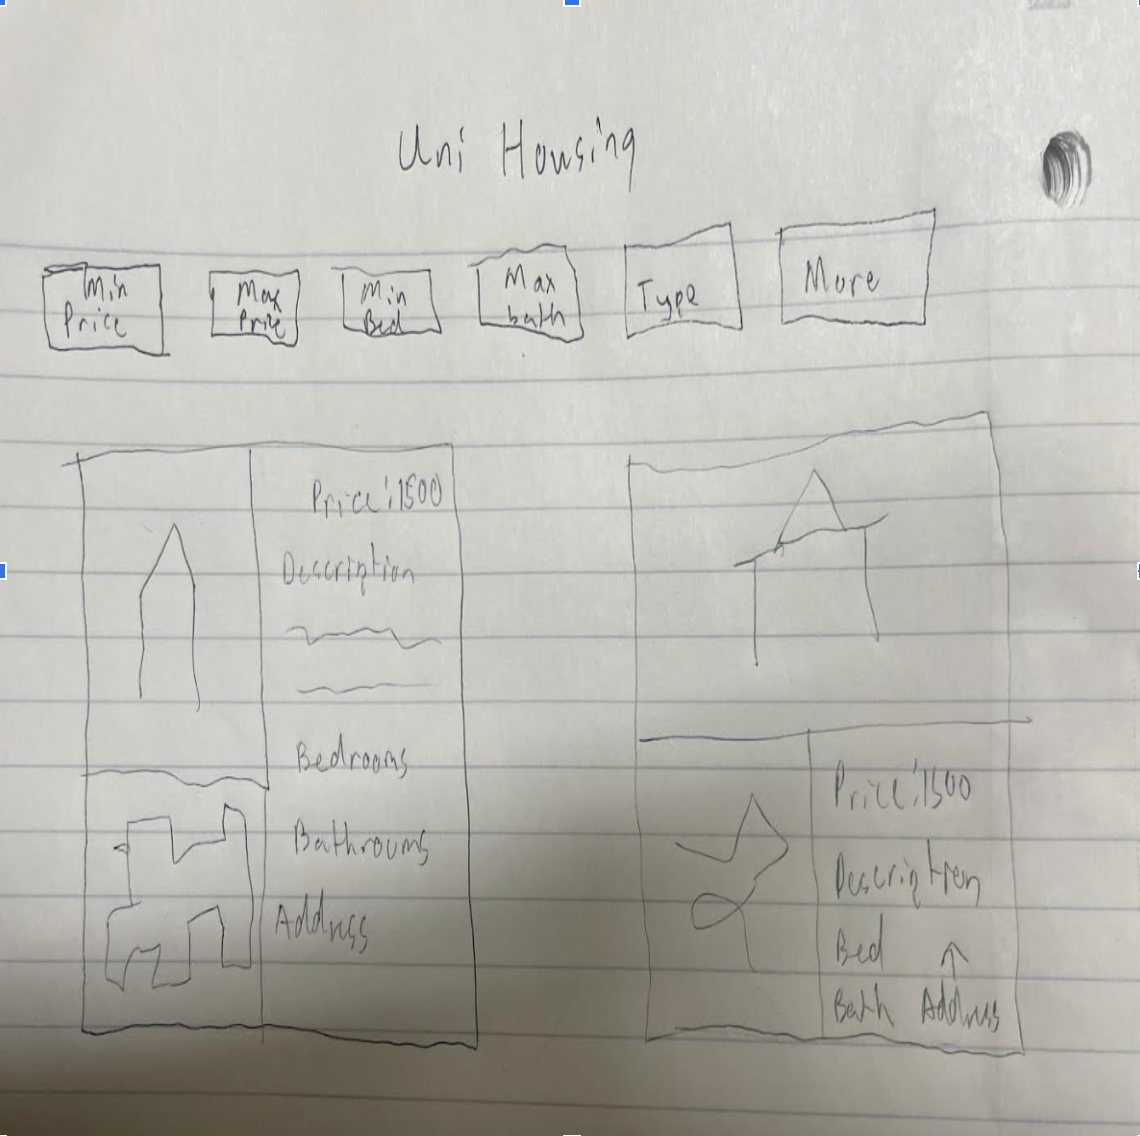
\includegraphics[scale=.35]{Early User Test.png}}

This phase of testing was primarily to ensure that when my react skills were good enough to create an actual design I had some insight into users preferred layouts and filters. While it was a bit difficult to provide an interactive experience for users I was able to draw enough information to aid in my initial designs. Most students only wanted one picture, and felt some filtering was redundant. The most important thing I may have learned from this however was how to do better testing. I found that my testing subjects would look to me for guidance when I was in the room, and in the interviews afterwards I could find myself asking leading questions to try and confirm my own beliefs. To limit this confirmation bias effect in the future I did my best to avoid asking leading questions and to get more unfiltered testing results, my testing process mirrored one of the following approaches for all subsequent tests. \\

\noindent• Watching the user use the application and observing without interference, asking the user not to speak to me until they felt they had fully completed their process \\ 
\textbf{OR} \\
• Having people use the application and leaving the room to allow them to use it in peace and then discussing their experience solely in the interview afterward, having them demonstrate to me if necessary.  \\

\subsubsection{User Testing - Website}
Over the next few months, once I had developed an adequate coding ability I was able to conduct testing on the actual sites I was beginning to build. This began with basic prototypes as seen below with limited filtering logic and untested (and unfinished) listing design.\\

\centerline{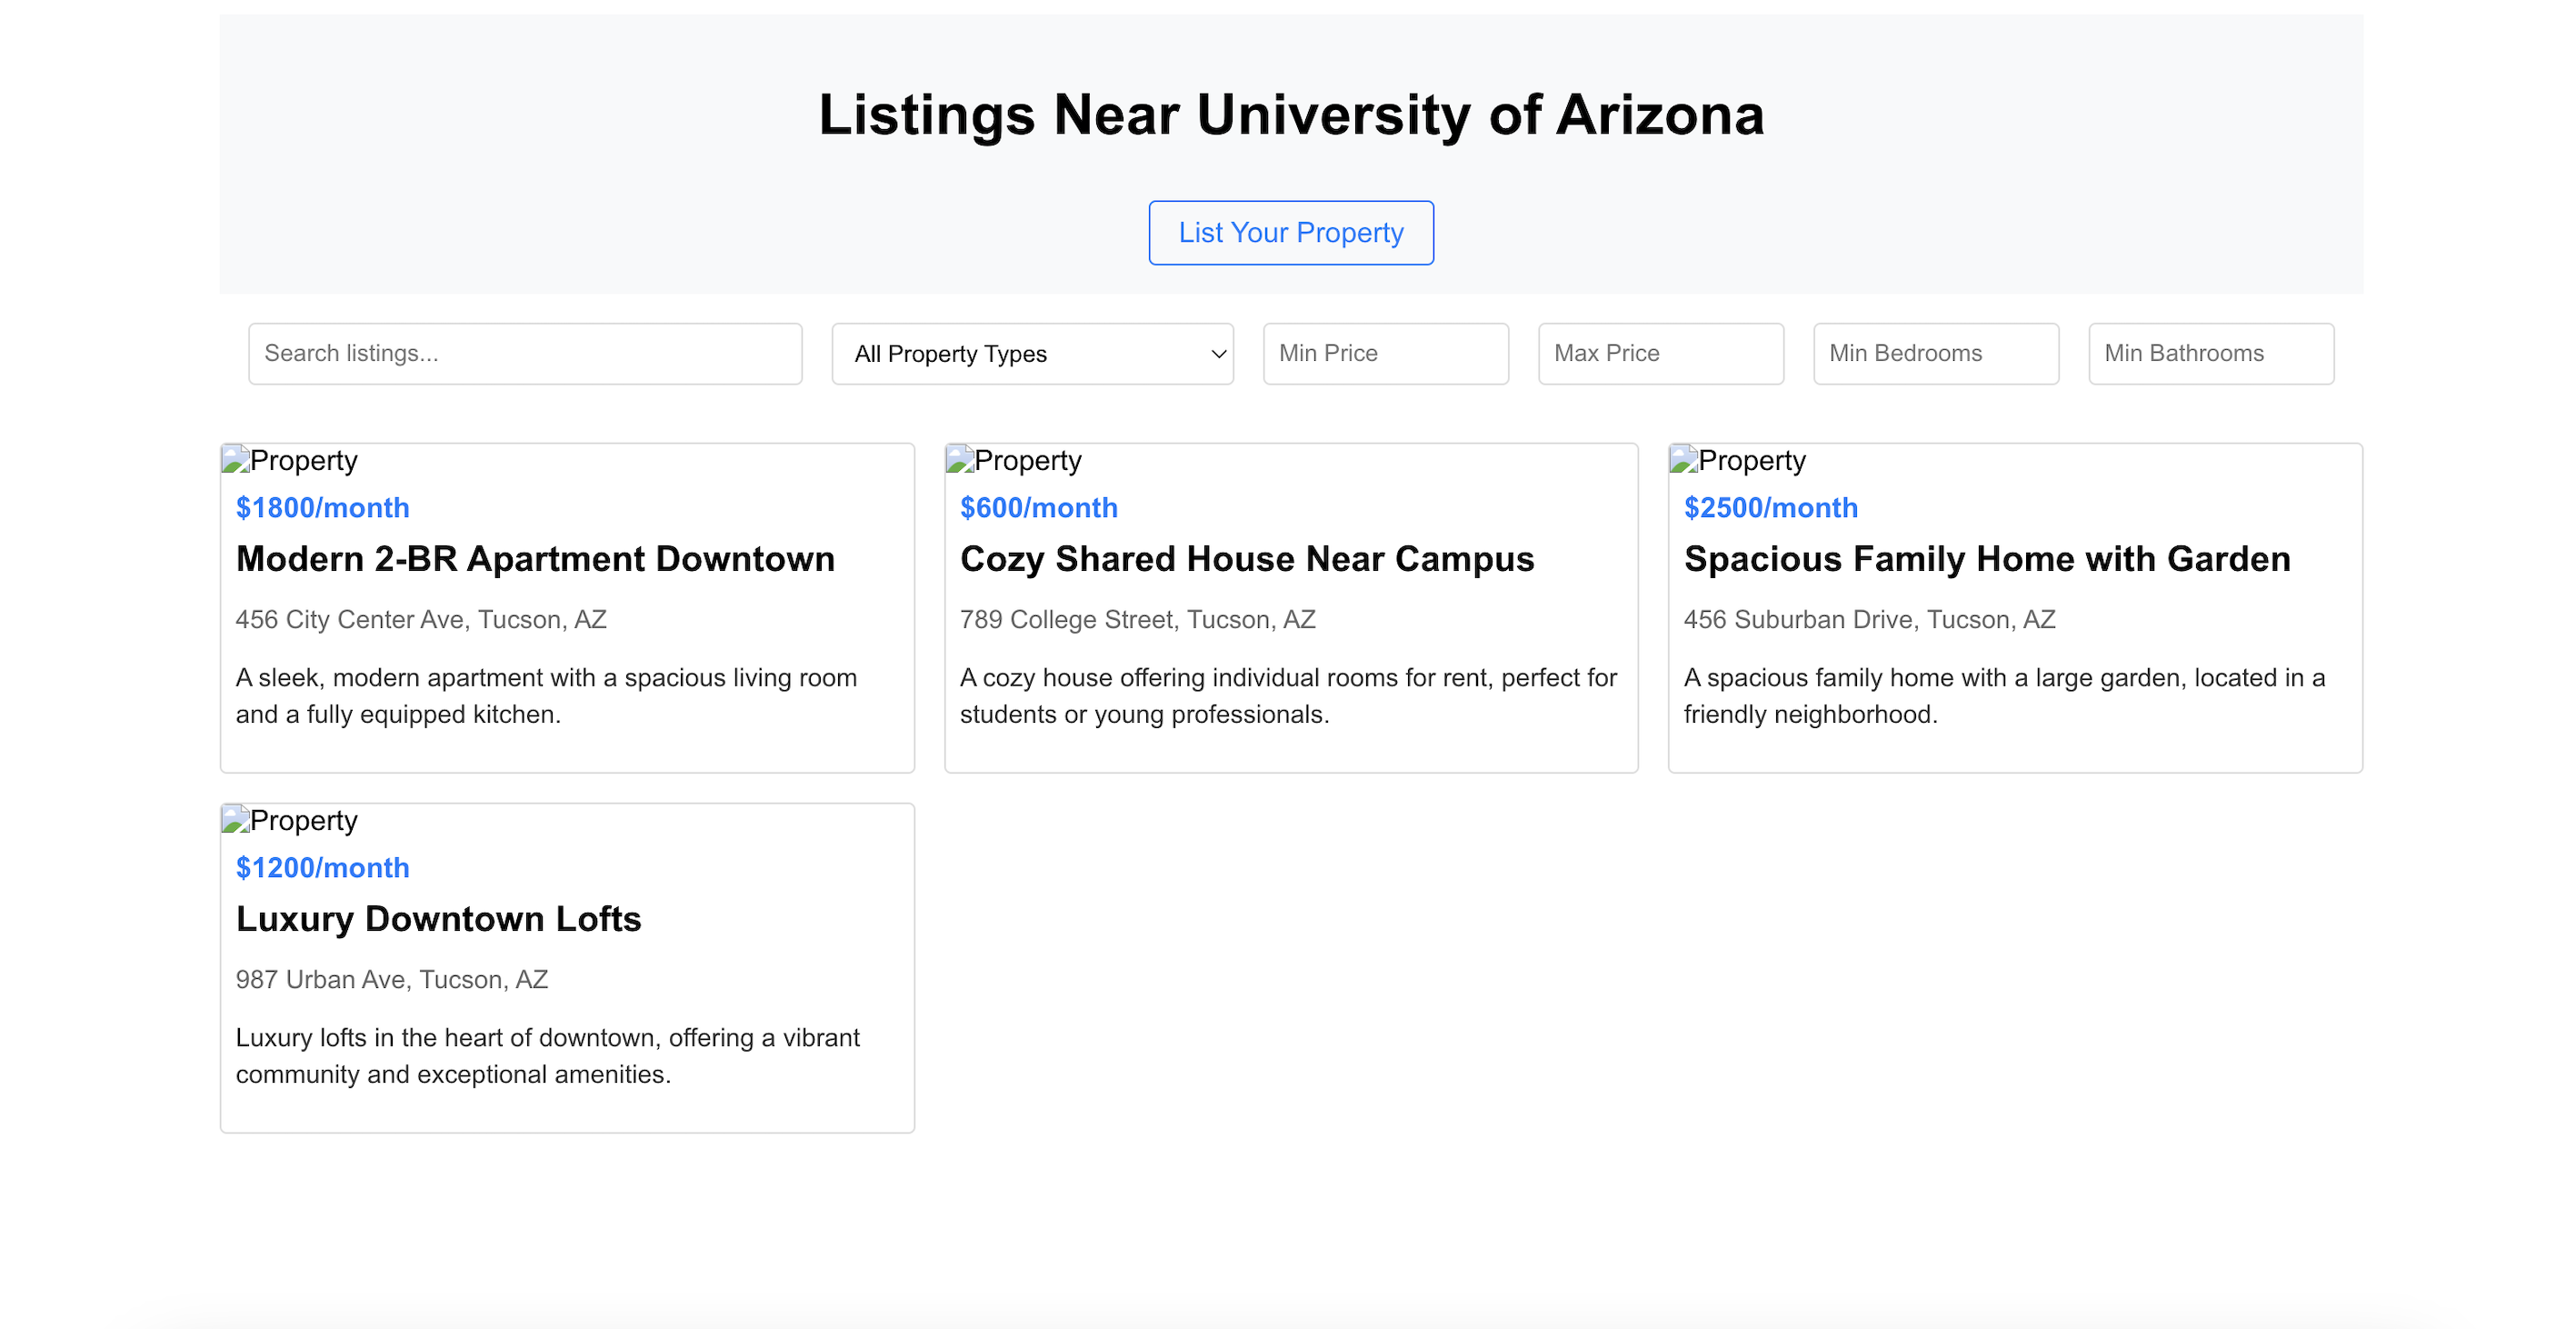
\includegraphics[scale=.15]{Old Screenshot.png}}

I did multiple rounds of user testing over the span of about 2 months following the approach I outlined above. While I did not let users directly make changes to the product, I valued their feedback and their responses provided valuable insight on what direction to take parts of the application. Highlighting the reasoning behind every decision I made is not practical given the length of the paper and some decisions will be covered in later sections; but some examples of key decisions I attribute to the iterative user testing/interview process are the filtering choices, inclusion of a maps API that allows users to identify how far away the property is from any other address, the ability to hide addresses on listings for the safety of property owners and the inclusion of room by room listings. These were so important because they had direct implications for improvements upon other applications, and were some of the most pertinent and significant concepts that users desired in an improved web app. In the end this process massively shaped the final product and was a significant portion of the methodology of my project.

\subsection{Technical Methodology}

\subsubsection{LocalHost Development}
 Originally, I intended to have a full scale application with databases to store the real listing data along with both landlord and renter accounts. This approach had a few problems. First my relative inexperience with my chosen languages made my learning curve fairly steep and limited what I felt I had time to focus on for the time constraints of the project.  When it came to creating a listing database, when room by room rentals became apart of the project it became clear that there were plenty of API's with rental listings but none for room rentals and it would require a vast amount of work to put together any kind of truly realistic database with room rentals. Lastly, not only did receive complaints about requiring accounts on the renter side, creating a database that took in sensitive information such as government issued identification and personal information like age of young women came with privacy concerns that I did not feel prepared to deal with, nor would they make any improvements to any of my stated goals. All current applications have vast privacy policies, while I could hope to implement those in the future, within the context of this project and my current skill set it was not a reasonable undertaking. \cite{airbnb_privacy} This led to me focusing on developing the front end of the application and running it only through a Localhost port for this project. 

\subsubsection{Front End Development}
As mentioned above the application is built using the React framework. React was chosen for its component-based architecture, which enables better organization of the code, easier debugging, and efficient rendering. This approach is in line with modern web development best practices and research on improving user experience. The user interface is clean and intuitive, featuring essential functionalities such as searching, filtering, and viewing property pictures. 

\subsubsection{Back End and Database Decision}
As covered above this project is focused on the front end development. I chose to focus on this side of development due to advice given to me throughout the project surrounding limiting my scope given my abilities, and because I felt it was the more important aspect of solving the housing \textit{search} process. This means that I do not cover things like user login or listing management that you would see in a full housing application. My listings page for example resets on submission because I had no real database to plug the information making it a relatively pointless endeavor to have it act as a entirely realistic submission. The larger issue is that college housing websites do not exist in a way that easily connects students looking for housing with information specific to college students needs. To me this meant that creating the front end/prototype of the platform was much more important to tackling the problem than the creation fully accurate databases, or the ability for someone to log in as there aren't large issues in that in other application that I would be solving. Also given that data like this could not be easily tapped into to provide relevant information for the project, it did not make sense to focus much on having a hyper-realistic database. This means that for "data" I created mock Listings that replicated real listings in a json file to display data on the listings page that would mirror what real data would look like. 

\subsubsection{Maps API}
In this project, the Google Maps Distance Matrix API is employed to enhance the user experience by providing real-time distance and travel time calculations. The API is integrated into the application's functionality to calculate and display the distances and estimated travel times between an inputted point of interest for the user. This means they can input any real address or location into the input box and it will provide them with the real time walking/driving distance and time. This API was chosen for its ease of use, along with its known accuracy in travel times. A visual representation of the API's use is seen below. \\

\centerline{\includegraphics[scale=.35]{Location.png}}

\section{Evaluation Metrics}

In order to evaluate the success of my college student housing app project, I primarily will use qualitative methods to measure the success of the application. The evaluation will be centered around the clarity of the applications use, ensuring both students and landlords can effectively manage their needs on the application. This will be primarily through my final user testing and interviews where I saw how users interact with the application, and ensure that it is easy for users to understand, along with taking feedback on if the application solves the identified problems with the current housing search for college students. After use of the application, I also asked questions about my product that emphasize comparing it to alternative applications to see how well my project accomplishes the goals I have set out. Some examples of questions from these final interviews are below. \\
What portions of the application did you find differed from other housing applications? Were they more useful? \\
Does this seem like an application you would use to find college housing, why or why not? \\
Were you able to find all information you wanted with relative ease? Is there something that was left out that you feel should be included in the housing search process? \\

Since this project is focused on the the front end and in particular the UI design of the application, ensuring the application is understandable and can help create an improved and more knowledgeable housing search process is the best way to evaluate its success. A full scale web application would usually have goals such as site visits to increase profitability or boost market share but I am able to focus on qualitative methods because I don't have any quantitative data anyway, and it provides a more nuanced connection with the user experience.\cite{belanger2006web} The lack of full functionality does limit me for now in the kinds of evaluation I am capable to performing, and if I expanded this into a full application I would certainly see the value in bringing in some statistical metrics, but given these constraints my user interviews remain my best option for effective evaluation. In my final analysis, by blending user testing and interviews, I believe I can achieve a comprehensive assessment that encompasses not only functionality but evaluates how effectively the platform fulfills its users' needs.


\section{Evaluation Results and Discussion}
\subsection{Original User Interviews and Testing - Contrasting Desires}
In my original conversations and paper testing what I found was that much of this projects difficulty was going to come from trying to serve two competing masters at the same time. Landlords wanted to give information but as little of it as possible in as simple of terms as possible. Multiple potential users ranted against the large sums of information often collected that felt irrelevant to a prospective renters decision. Many of these conversations led to the realization that one of the main improvements that could be made for property owners is the ability to clearly list rooms individually as they felt no applications truly did this effectively.\\

On the other side of the coin I needed to serve the needs of college students as they would be my primary users. What they denoted was that housing apps are good but having something with listings near colleges would be particularly helpful. They focused on the usability of the app, disliking accounts, wanting to implement specific filters like leasing dates and different rental types such as room rentals, while eliminating redundant filters seen on other housing applications. They also wanted to know a significant amount about the property, "the more the better" was thrown around a few times so one of my biggest challenges was finding a way for landlords to quickly display amenities that users could want to interact with. 
\subsection{Web Application/User Testing}
The development of the applications interface was an equally important portion of the project as understanding user needs. Making sure that users were comfortable with the design and could easily understand how to interact site. This meant making decisions on key components such as listing cards per line, what to display on each card and how things like pictures, contact information and the distance feature could be best implemented in the interactive portions of the app. This led to thoughts about what information was most important to be displayed up front, how did users interact with the application to get other information they desired. 

\subsection{Final Results - Project Goals}
To assess the effectiveness of my final product in meeting my project goals, I focused on conducting a final round of user testing and interviews to understand how the project connected with my stated goals. While I took an iterative approach in the creation of the application meaning it was evaluated at many steps in the development process, I felt evaluation the final product was the appropriate thing to assess in this paper. I conducted 3 interviews on the property owner/manager side and 8 on the renter side. I would have preferred to conduct more particularly on the owner side to have more input but I was limited by who I know who owns property in college markets on the owner side and by what students were willing to take time away from finals on the student side. Participants engaged with the platform and I instructed them to focus on the usability of the current front end interface rather than missing components that would make it a full scale application as my goals within the project were to develop an improved front end.

\subsubsection{Property Owners}
I received extremely positive feedback from homeowners on the site, they liked the direct to listing approach from its outset and felt the listing page was easily accessible with the design of the List Property button standing out on the ListingsPage. While many acknowledged there was no account information the design of the page to list the property was ideal particularly for the owners looking at the room by room rentals as it quickly allowed for labeling of bedrooms along with providing the necessary information for the user about each individual bedroom. I received positive comments about the changes to amenities, allowing them to type it in as a comma separated list past a few key amenities was far more desirable than spending time clicking through countless boxes of possible amenities that could not be appropriately regionally limited with my skill set. Additionally, I gave them plenty of time to freely interact with the application so a couple looked at the Listings Page and had positive feedback on its design and enjoyed seeing the implementation of the features coming through in the listings such as addresses not being displayed. 

\subsubsection{Renters}
The feedback I received from college students was insightful and demonstrated how the changes I had made from a traditional housing application. Each of these students was an upperclassmen and had experience going through the housing search which is what I preferred because it gave them the opportunity to compare to previous housing sites they had experience with. I once again received beneficial feedback which greatly supported the goals of my project. Students expressed that they liked the user interface particularly the spacing and the intuition of the design as it was similar in use to other applications. When it came to the changes made from other applications filter changes for lease date starts were particularly appreciated by those who simulated a summer housing search. The listing cards were a source of a bit of mixed feedback. Some suggested implementing a contact button on the card and not solely in the Listing Detail page but a majority felt it would have made the cards to cluttered and remarked that it was unlikely anyone would call about a property before looking into greater detail that was only available to be displayed in the listing detail page. Throughout the interviews most also supported  the filter choices, although many respondents from Arizona wanted pool to be included. Given this seemed like a very regional choice, those based in California and Oregon never once responded asking about a pool I felt it best to leave it as something in the amenities section and possibly add the ability to search based upon amenity in future works. Additionally some lamented the lack of a map while some actually preferred its disappearance as they felt it allowed better viewing of the listings and they could still use the Distance Calculator to discover how far away a property was from different locations.  

\subsubsection{Goals}
If you will recall a narrow summary of my goals was to enhance the college search process for students by providing them with a site that met their unique needs, while providing landlords ways to more effectively access the college market. As you can see the questions I asked surrounding my goals during final user testing were responded to relatively positively. Property owners in college markets were happy to see that they had options in how to list potential properties and that the process was not cumbersome, frequent comments were made about how the time to list was similar to a Craigslist listing than an Air Bnb listing. I felt this feature may do more to attract additional landlords who were looking for an easier listing experience.\\
On the student side I was pleased because the responses I received acknowledged that the changes made to the front end I created were similar to the changes students desired to their housing search.  While my design is not as beautiful as Air Bnb for example, users noted that it was effective at conveying necessary information and retained the useful attributes of other housing applications which made my apps use very intuitive. At times I received mixed feedback on filtering priorities, and given more time I would certainly spend time finding ways to filter by amenities in a way that would keep the property listing page in its current form. Overall I felt as though these final user tests demonstrated that the created front end would be seen as useful by many users and if implemented in a fully developed application would solve many of the issues with current sites which I have identified over the course of the paper. 

\subsection{Caveat/Future Work}
This app is obviously very limited in its design. Given the time frame, my naivety with my chosen project and corresponding programming languages, along with the requirements of the project there is a lot left to be desired from this becoming a full scale application that could be deployed as an actual housing app. I think there are two primary sections that I would expand on if I continue this in the future, a true database along with addressing privacy and security concerns.

\subsubsection{Real Data!}
The first step I would like to take in the future is implementing real data into my listings so that users could interact with actual rental listings. I am still a bit unclear on how to precisely achieve that due to the lack of an individual source for room listings. Through some research I believe I have found some approaches that would work. To transition from our mockListing.json file to real housing listings, I would begin by sourcing data from property owners, real estate agencies, or public APIs that provide actual housing listings. Data validation procedures would need be put in place to maintain the accuracy of the data. I would need to decide on what database tools would be used to store this data. Another large issue I would need to cover is that regular data maintenance processes would keep the database up-to-date to ensure rentals that have been rented do not remain on the market. This simple explanation demonstrates a relatively comprehensive future approach would enable the platform to provide users with reliable and current real housing listings.


\subsubsection{Privacy and Security} 

As the developer of a web app designed to help college students find housing, I recognize a large consideration in the creation of this app is the paramount importance of ensuring the privacy and security of my users' personal information. Air Bnb, likely the most popular rental applications that exists today has a massive privacy policy for good reason, this level of security and privacy gives them legitimacy they need to operate a business that has massive impacts on individuals everyday safety. \cite{airbnb_privacy} This is especially crucial for young women, whose physical safety could be jeopardized by inadequate security measures by a web application giving away information about their possible housing location. I shied away from some of these questions in this application as I narrowed the scope of the project, and incorporated user feedback about how to keep individuals secure. One of my biggest regrets that came as a result of my final user tests where a homeowner mentioned that in its current form anyone could access this site. This is fine given the current nature of the application not existing outside of this project, but as I continue to build it I would like to see it grow into a real product and would need to solve that as quickly as possible. To ensure my app could exist solely for students, and not infiltrated by just anyone looking for rental housing or by those who desire to use this app for creepy purposes such as living with college students I would need to take appropriate measures. A suggestion I received to address this issue that I found useful was to ensure accounts are verified with emails that are attached to a school or university, or requiring a school ID be uploaded and verified in the application. These emails for example are only given to students and are usually shut off one to two years after a students graduation making them an ideal way to verify age and attendance and school ID's typically denote a graduation year. This is something I would certainly add as I continue to work on this in the future to ensure my users are getting a product that keeps them safe.  

\section{Ethical Considerations}

Creating a project like this comes with questions surrounding ethical development when creating the application. Developing an online space to provide college students an easy way to search for housing requires a commitment to moral and social considerations, fairness and transparency, unbiased promotion and user safety both physically and digitally. By confronting these moral quandaries, I will be able to create a platform that benefits both college students and the wider community, promotes equity and access, all while disrupting the college housing market.

\subsection{Transparency and Discrimination}
Fairness and transparency are crucial ethical considerations when developing an app to provide a space for college students to find housing. As the developer, I recognize that housing is a fundamental need, and access to fair and affordable housing is essential for a healthy and equitable society. In other housing apps it is very common to receive some kind of push back or refusal of sale when the owner of the property discovers the students age which prolongs the housing search. I do not think this app can erase the stigma associated with renting to college students, but it can give college students immediate access to willing homeowners giving them a leg up on the housing search in their area and providing access to a lucrative market for those landlords who put their properties on the application. To promote fairness and transparency, I implemented certain features that prevent discriminatory practices, such as bias against certain races, genders, or socioeconomic backgrounds. I hope to provide a more neutral setting for the promotion of properties than is seen in other applications. Programs like Air Bnb or Vrbo use algorithms to promote certain properties and hosts. However the design of their page and algorithms are shown to promote white hosts and customers tend to favor hosts with whose pictures appear to be white at the expense of people of color.\cite{jaeger2020racial} To promote fairness and eliminate discrimination, I did not include any information about race, and did not display pictures of landlords or require them to attach their name to the listing. This means that the app does not collect or use any demographic data, such as race or ethnicity, in the matching process. Instead, the app allows the student to use objective criteria such as location, price, and amenities to filter their housing options. I also believe it's important to provide clear and accurate information about housing listings and rental agreements so that users can make informed decisions. I want to avoid becoming similar to ticketing apps that hide fees, or hotels who seem to find a new "resort tax" to add onto your bill each time you make a reservation. This means property owners will have to list \textbf{all} pricing information about their property on the website, this includes monthly rent, security deposit and whether utilities are included in the price or if they are an additional cost. This allows users to make informed financial decisions before even considering contacting the owner about a possible living space. By avoiding this partitioned pricing model some studies believe I can actually retain more users, and at the same time I will uphold my ethical standards. \cite{greenleaf2016price} By following these guidelines and prioritizing fairness and transparency, I aim to promote a housing search process that is equitable for all users, regardless of their backgrounds or circumstances. 

\subsection{Legal Issues}
In the course of this application I ran into quite a few ethical conundrums that also coincided with legal issues that I felt were necessary to address. For example I would have loved to include the ability to upload sign-able rental agreements easily on the website but in doing so I open the application up to litigation if a property owner does not meet the obligations of the lease agreement. Instead I require government ID, phone number and email so that if this app were developed into a full scale application, under the scenario of a landlord not meeting their obligations I would have information on hand to provide the renter on how to seek retribution. Another issue like this came to whether I can confirm that rooms that are listed individually have locks on the doors. Unfortunately through the app I don't have much of a way to ensure this, so much of the burden is passed to the potential renter to verify the property matches the listing, however that could be the case for any information a landlord posts about a property on any site so I am comfortable with that. 

Another legal/ethical question that came up was whether I was able to list gender in the occupants of current rooms for room by room listings. What I found was that in most cases you are indeed able to denote the gender of the current occupants due to the Federal Fair Housing acts language on shared common spaces.\cite{fairhousingact} This gave me the ethical question of what is the right thing to do for my users, is that information I should make available or is that something I am obligated to keep private as some would prefer that information not to be shared? What I decided through conversations with both users and homeowners is that information should remain private. This is primarily to protect the safety of dwellings with only young women living in them for example, publicly broadcasting that any home is only occupied by women could become a safety issue for occupants for a variety of obvious reasons. Through my user conversations I found that in most room by room cases property managers would try to match by gender anyway, and if a homeowner wont tell a prospective tenant the gender of their possible roommates, that is a warning sign that would likely drive someone away from possibly renting the property. 


\section{Conclusion}
This project examined ways to address issues with the housing search process for college students. Despite the shortcomings and narrowed scope discussed, I believe that the project succeeded in meeting the goals that I set out to accomplish. My main task was that users on both sides of the rental process would see this process improved by tailoring it to this niche market. From my evaluations it became clear that students and homeowners both saw benefits from the design of the application indicating the utility I desired. I believe that this reinforces the importance of finding ways to continue to refine this process as the housing crisis is disproportionately impacting college students. Overall I feel the current state of the project, along with extensive user testing results shows that the current design of this application would be useful to a finished college rental application. 


\appendix
\section{Replication Instructions}
Follow these instructions if you wish to view and run the project locally on your machine. \\

\noindent Prerequisites:
Install node.js and npm from the Node.js website - https://nodejs.org/en
Npm (the package manager) is automatically included with the node.js download. \\
\\
Go to terminal and check that both are installed with commands:\\
node -v \\
npm -v \\

\noindent I am using node v18.16.0 and npm v9.5.1 \\
\\
Use git to clone the project with this command: git clone https://github.com/wiermanc/Uni-housing.git\\
\\
In terminal change your root directory to the projects with the command: cd Uni-housing \\
\\


API Key - you will also need to obtain an api key in order to effectively test the distance function. \\

Obtain a Google Maps API Key:\\
Visit the Google Cloud Platform Console.\\
Create a new project.\\
Navigate to the "APIs \& Services" dashboard.\\
Click “Enable APIs and Services” and enable the “Distance Matrix API” or "Routes API".\\
Go to “Credentials”, then “Create Credentials”, and select “API key”. \\
Once your API key is created, Copy the API key for use in the project. \\
Open the ListingDetailPage.js with the command: nano src/pages/ListingDetailPage.js\\
Find the old (disabled) API key denoted by the variable const apiKey, which is in line 28 at the time of writing and replace it with your new API key\\
After making the change, save the file by pressing Ctrl + O, then press Enter to confirm.\\
Exit nano by pressing Ctrl + X.\\
It is not usually recommended to have the API key so easily accessible, but considering this project is only to be run locally this organization is fine for now. If you are trying to expand this further you may need to consider changing the location of the API key to prevent possible security concerns. \\

Install the necessary dependencies by running: npm install\\
\\
At this point you should be able to run the application on your localhost:3000 port and it should pop up in your browser. Achieve this by running: npm start \\




\section{Code Architecture Overview}


Overview:

The codebase for my Uni-housing application is organized to promote readability and maintainability. The code is thoughtfully arranged into specific sections, each designed to handle a different part of the app's features. This setup ensures that everything is in its place, making the code intuitive to navigate and work with. This approach is evident in the four main components: ListingsPage, ListingDetailPage, ListingCard, and FilterBar.

ListingsPage is the epicenter of the application, serving as the main container for the listing summaries. It integrates FilterBar, which encapsulates the filtering logic, allowing users to decide upon their search criteria. The ListingCard is a sub-component used within ListingsPage to display individual listings in a concise format. These cards are interactive and, upon user click, navigate to the ListingDetailPage, which provides a detailed view of the selected listing.

While I believe the code to be fairly straightforward for any developer with the skill to continue building upon it there are sections with comments to ensure understanding of the code, particularly those related to filtering and sorting listings, have some comments to assist anyone examining the code. Mainly each filter is labeled so that it is easy to understand what each block does. This not only aids in understanding the code's current state but also streamlines the debugging and extension processes for future developers.

Diagram:

A comprehensive diagram can be seen below, providing a visual representation of the application’s architecture. This diagram delineates the flow of data and user interactions, clarifying the relationship between components and the sequence of events triggered by user actions. The use of distinct shapes in the diagram aids in distinguishing between different types of components, with arrows illustrating the direction of data flow and user navigation.

\centerline{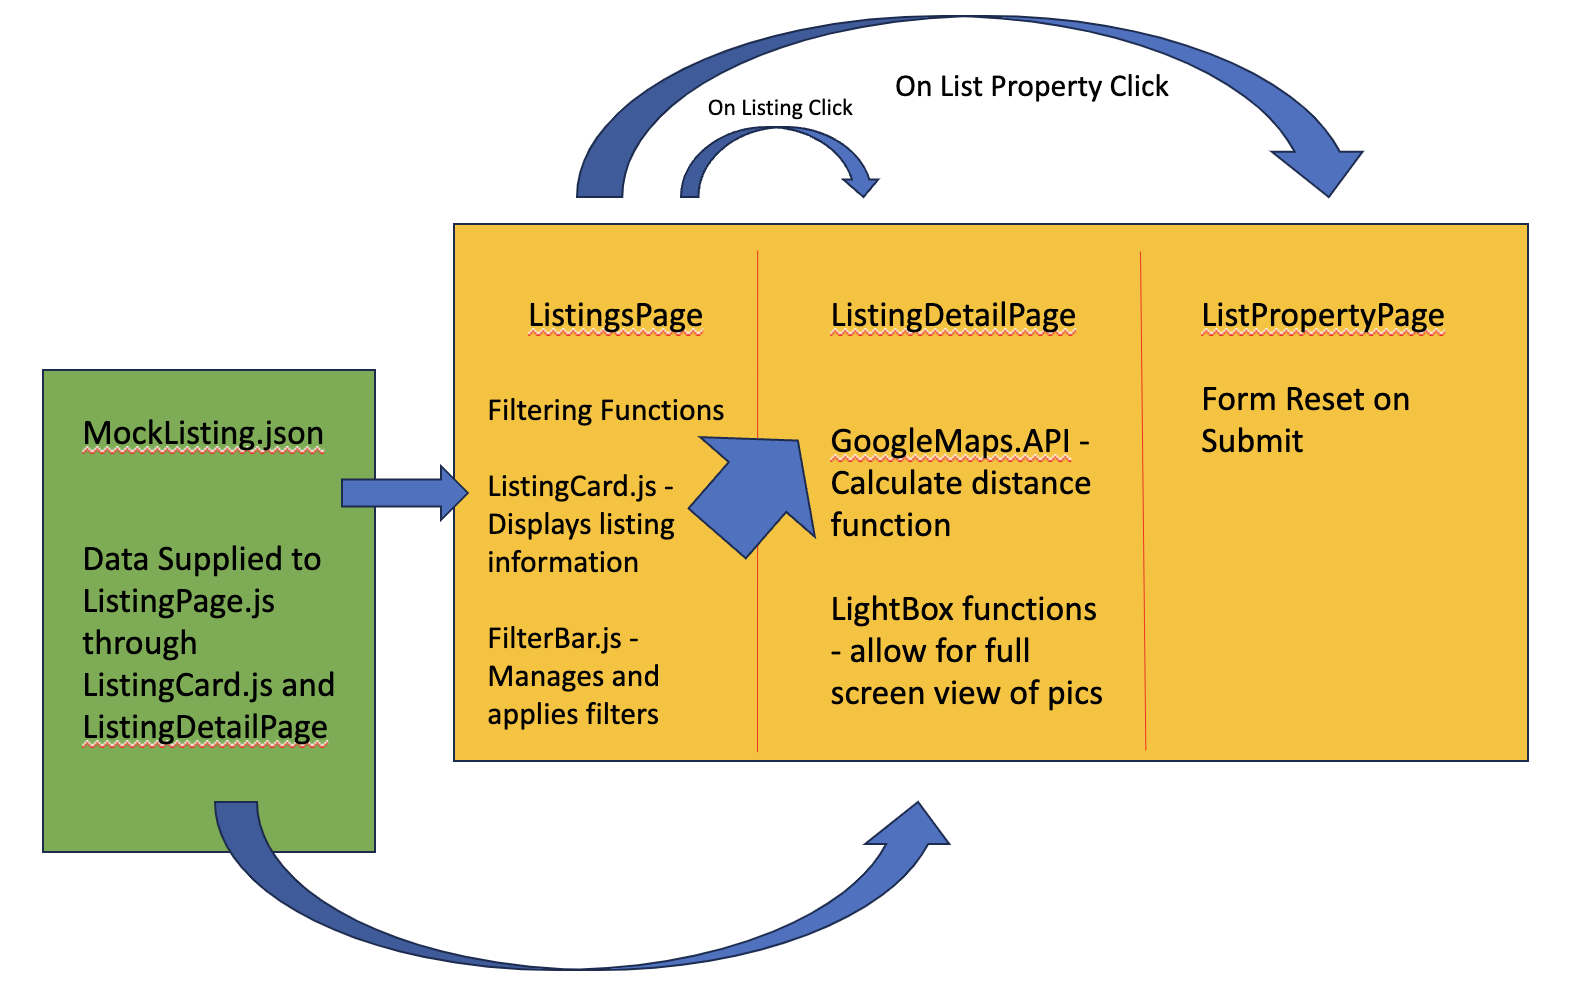
\includegraphics[scale=.35]{Code Architecture.png}}

Future Extension and Debugging:

The clear separation of responsibilities among components means that extending the application is straightforward. For instance, should new listing features need to be implemented, developers can easily identify the ListingCard component for UI changes, or the FilterBar for adjustments to search criteria.

Debugging is facilitated by the logical flow and state management within the ListingsPage. Since it acts as the source for listing data, developers can trace issues back to this centralized node, reducing the complexity typically associated with diagnosing state-related bugs.

Conclusion:
The code's organization, coupled with detailed comments and a clear architectural diagram, ensures that any developer—whether they aim to extend the application with new features or troubleshoot existing functionality—will find a well-documented and logically structured code base to work with. 
\clearpage
\printbibliography
\end{document}
